%QCM pourcentages / proportions / taux d'évolution / évolutions réciproques

\section{Questions à choix multiple \textit{(6 points)}}

Cet exercice se présente sous la forme d'un questionnaire à choix multiple (QCM). Les six questions sont indépendantes. Pour chaque question, une seule réponse est exacte, on demande d'indiquer cette réponse sur la copie sans la justifier. Chaque bonne réponse rapporte 1 point, chaque réponse incorrecte retire \num{0.25} point, une question sans réponse n'apporte ni ne retire aucun point. Si le total est négatif, la note est ramenée à 0.
%On inscrira sur sa copie, le numéro de la question et la lettre de la réponse choisie.
\vspace*{0.5cm}

\begin{questions}
	\question[1] La population d'une ville est de \num{30000} habitants. Si elle augmente de 15 \% par an, quel sera le nombre d'habitants de cette ville dans deux ans ?
	
	\begin{oneparchoices}
		\choice \num{30675};
		\choice \num{39000};
		\choice \num{35175};
		\CorrectChoice \num{39675}.
	\end{oneparchoices} 

	\question[4] Une enquête est menée auprès de 250 personnes a donné les résultats suivants :
	
	\begin{center}
		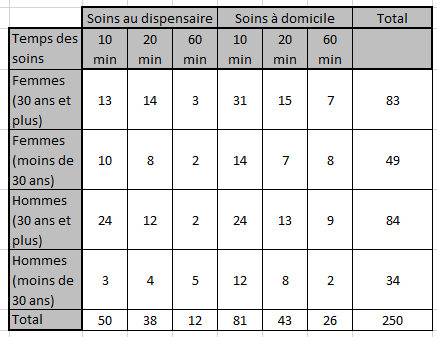
\includegraphics[scale=0.5]{img/soins}
	\end{center}
	
	\emph{Tous les pourcentages donnés ci-dessous sont 	arrondis à 1 \%.}
	\begin{parts}
		\part[1] Quel est le pourcentage des hommes ?
	
		\begin{oneparchoices}
			\correctchoice 47 \% 
			\choice 34 \%
			\choice 14 \%
			\choice 79 \%
		\end{oneparchoices}
	
		\part[1] Quel est le pourcentage des personnes qui reçoivent des soins de plus de 15 min ?
		
		\begin{oneparchoices}
			\choice 25 \% 
			\choice 40 \%
			\correctchoice 48 \%
			\choice 53 \%
		\end{oneparchoices}
	
		\part[1] Parmi les femmes, quel est le pourcentage de celles qui se font soigner à domicile ?
		
		\begin{oneparchoices}
			\choice 58 \% 
			\correctchoice 62 \%
			\choice 65 \%
			\choice 70 \%
		\end{oneparchoices}
	
		\part[1] Parmi les personnes qui se font soigner à domicile, quel est le pourcentage des hommes ?
		
		\begin{oneparchoices}
			\choice 15 \% 
			\choice 31 \%
			\correctchoice 45 \%
			\choice 79 \%
		\end{oneparchoices}
	\end{parts}

	\question[1] Dans les cas suivants, quels sont les taux d'évolution réciproque l'un de l'autre ?
	
	\begin{oneparchoices}
		\choice 30 \% et - 30 \%
		\CorrectChoice 25 \% et - 20 \%
		\choice 150 \% et - 50 \%
		\choice 60 \% et - 40 \%
	\end{oneparchoices}
\end{questions}  